\documentclass{article}
\usepackage{pgffor}
\usepackage{filecontents}
\usepackage{pdfpages }
\usepackage{graphicx} 
\usepackage{a4wide}
\usepackage{here} 
\usepackage{tabularx}
\usepackage[colorlinks]{hyperref}
\usepackage[german]{babel}
\usepackage[utf8]{inputenc}
\usepackage[T1]{fontenc}
\usepackage[3D]{movie15}
\usepackage{booktabs} 
\usepackage{eurosym}
\usepackage{verbatim}
\usepackage{amsmath}
\usepackage{textcomp}
\usepackage{caption}
\usepackage{setspace} 
\usepackage{geometry}
\usepackage{pdfpages}
\geometry{a4paper, top=25mm}

\setcounter{tocdepth}{5}  % Ebenen für Aufnahme in das Inhaltsverzeichnis
\setcounter{secnumdepth}{4}  % Ebenen für Nummerierung


\begin{document}

\begin{titlepage}

\begin{center}


% Oberer Teil der Titelseite:
\includegraphics[width=0.15\textwidth]{./Files/logo.png}\\[1cm]    

\textsc{\LARGE Zwischenbericht}\\[1.5cm]

\textsc{\Large Bremen}\\[0.5cm]


% Title
\newcommand{\HRule}{\rule{\linewidth}{0.5mm}}
\HRule \\[0.4cm]
{ \huge \bfseries Team Gamma}\\[0.4cm]

\HRule \\[1.5cm]

% Author and supervisor
\begin{minipage}{0.4\textwidth}
\begin{flushleft} \large
\emph{Autoren:}\\
Robin \textsc{Bley}\\
Alexander \textsc{Brennecke}\\
Alexander \textsc{Feldmann}\\
Marc \textsc{Huisinga}\\
Kevin \textsc{Neumeyer}\\
Till \textsc{Schlechtweg}\\
Steffen \textsc{Wißmann}
\end{flushleft}
\end{minipage}
\hfill
\begin{minipage}{0.4\textwidth}
\begin{flushright} \large
\emph{Betreuer:} \\
Harm \textsc{Hörnlein-Roboom}\\
Frank \textsc{Marschall}
\end{flushright}
\end{minipage}

\vfill

% Unterer Teil der Seite
{\large \today}

\end{center}

\end{titlepage}

\newpage
\thispagestyle{empty}
\tableofcontents
\thispagestyle{empty}
\newpage
\setcounter{page}{1}

% Import des Kurzberichtes
\section{Kurzbericht}
In den vergangenen Monaten haben wir uns damit beschäftigt, unser Projekt fertigzustellen und durchzutesten. \\
Im Bereich der Hardware sind bereits der Fallschirm, die Einrichtung unseres Mikrocontrollers, die eigentliche Dose, die Sensorik, die eigentliche Sensorikplatine, das Innere der Dose und die Antenne fertiggestellt. Aktuell beschäftigen wir uns mit der Integration der Komponenten. Einige Bereiche sind bereits durchgetestet, während andere Bereiche, welche das fertige Gesamtsystem erfordern, aktuell noch getestet werden. \\
Die Desktopapplikation ist mittlerweile komplett fertiggestellt und wird lediglich noch getestet und an einigen Stellen verbessert. Es ist möglich, die Daten, beispielsweise mithilfe einer dreidimensionalen Kartenvisualisierung oder eines Graphen, darzustellen. Die Benutzeroberfläche kann beliebig angepasst und konfiguriert werden. Eines der wichtigsten Features ist die Kompatibilität zu anderen CanSats. Über die Benutzeroberfläche ist es möglich, beliebige CanSats und Übertragungsformate zu integrieren. So kann unsere Desktopapplikation auch von anderen Teams genutzt werden. \\
Zu der Android-Applikation werden aktuell noch weitere Features hinzugefügt. Sie ist dazu in der Lage, Daten über einen Hotspot von der Bodenstation zu beziehen und diese Daten in der Applikation mithilfe von Graphen darzustellen. Hinzugefügt wird noch die Möglichkeit, fehlerhafte Daten herauszufiltern und Einheiten in den Graphen anzuzeigen. Die Android-Applikation wurde bereits ausgiebig getestet. \\
Aktuell sind wir also dabei, die Hardware zu integrieren und das Gesamtsystem ausführlich zu testen, was darauf schließen lässt, dass das Projekt sehr bald als abgeschlossen erklärt werden kann.

% Import der Aufgabenliste
\section{Aufgabenliste}

\subsection{Aufgabenliste Hardware}
\begin{table}[H]
  \centering
    \begin{tabular}{p{3cm}p{7cm}p{3cm}rrr}
    \toprule
    \textbf{Aufgabe} & \textbf{Unteraufgabe} & \textbf{Status} \\
    \midrule
	Planung & Erstellung Verteilung der Arbeitspakete & abgeschlossen \\
	& Erstellung von PAP und PSP & abgeschlossen \\
	\midrule
	Bergungssystem & Fallschirmdesign entwickeln & abgeschlossen\\
	& Bau der Fallschirme & abgeschlossen\\
	\midrule
	Antenne & Antennendesign entwickeln & abgeschlossen \\
	& Bau der Antenne & abgeschlossen \\
	\midrule
	Sensorik & TMP006 testen und Codeentwicklung & abgeschlossen\\
	& Adafruit GPS testen und Codeentwicklung & abgeschlossen\\
	& BMP180 testen und Codeentwicklung & abgeschlossen\\
	& Sparkfun UV testen und Codeentwicklung & abgeschlossen\\
	& Transceiver testen und Codeentwicklung & abgeschlossen\\
	& Geeignete Stromversorgung entwickeln & in Bearbeitung\\
	& Sharp Feinstaubtest und Codeentwicklung & abgeschlossen\\
	\midrule
	Beagleboard & Auswahl der Programmiersprache & abgeschlossen\\
	& Aktualisieren der Software auf dem Beagle & abgeschlossen\\
	\midrule
	Dosendesign & Dosendeckel anfertigen & abgeschlossen\\
	& Ummantelung der Dose anfertigen & abgeschlossen\\
	& Dosendesign innerhalb der Dose & abgeschlossen\\
	& Platzmanagement in der Dose & abgeschlossen\\
	& Kabelmanagement in der Dose & in Bearbeitung\\
	& Stabilitätstest der Dose & ausstehend\\
	& Befestigung des Landungssystems an der Dose & in Bearbeitung\\
	& Löten und Integration aller Komponenten & in Bearbeitung\\
  \midrule
  Dokumentation & & abgeschlossen \\
  \bottomrule
  \bottomrule
  \end{tabular}%
  \label{tab:aufgabenliste_hardware}%
\end{table}%

\subsection{Aufgabenliste Software}
\begin{table}[H]
  \centering
    \begin{tabular}{p{3cm}p{7cm}p{3cm}rrr}
    \toprule
    \textbf{Aufgabe} & \textbf{Unteraufgabe} & \textbf{Status} \\
	\midrule
	Oberfläche & Verwaltung von Satelliten & abgeschlossen \\
	& Menüs für die Handhabung von Features & abgeschlossen\\
	& Option zum Auswählen der Location des Log-Files & in Bearbeitung\\
	& Icons zum Starten und Stoppen von Verbindung zwischen Clients oder Satelliten & abgeschlossen \\	
	\midrule
	Visualisierungen & Graphenvisualisierung & abgeschlossen \\
	& Kartenvisualisierung & abgeschlossen \\
	& Tabellenvisualisierung & abgeschlossen \\
  & Graphenvisualisierung Android & abgeschlossen \\
	\midrule
	Datenexport & Export für Daten im JSON-Format & abgeschlossen \\
	& Export für Daten im CSV-Format & abgeschlossen \\
	& Export für Daten im TXT-Format & abgeschlossen \\
	& Export für Daten im KML-Format & abgeschlossen \\
	& Daten-Logger für das JSON-Format & abgeschlossen \\
  & Logging auf Android & in Bearbeitung \\
	\midrule
	Datenimport & Daten aus CSV-Dateien importieren & abgeschlossen \\
	& Daten aus JSON-Dateien importieren & abgeschlossen \\
	\midrule
	Datenverarbeitung & USB-Schnittstelle & abgeschlossen \\
	& Input-Pipeline & abgeschlossen \\
  & Weiterleitung an Android & abgeschlossen \\
  & Empfang von Hotspot & abgeschlossen \\
	\midrule
	Tests & Automatisierte Tests für alle Exporter & abgeschlossen \\
	& Automatisierte Test für alle Importer & abgeschlossen \\
	& Automatisierten Test für Input-Pipeline & abgeschlossen \\
	& Testen der Netzwerkverbindung zwischen Bodenstation und Clients & abgeschlossen \\
	& Testen der Verbindung zwischen Bodenstation und CanSat & in Bearbeitung \\
	\midrule
	Architektur & Exporter in Input-Pipeline einbinden & abgeschlossen \\
	& Importer in Input-Pipeline einbinden & abgeschlossen \\
	& Visualisierungen in Input-Pipeline einbinden & abgeschlossen \\
	& Oberfläche mit Input-Pipeline verbinden & abgeschlossen \\
	\midrule
	Anpassungen & Verbindung zwischen KML-Visualisierung und Oberfläche überarbeiten & abgelehnt \\
	& Ausstattung einiger Visualiserungen mit Autoscroll & abgeschlossen \\
	& Kartenvisualisierung überarbeiten & abgeschlossen \\
	& Datenquelleninitialisierung der Input-Pipeline überarbeiten & abgelehnt \\
	& Quellcode-Dokumentation anpassen & abgeschlossen \\
	& Software-Architektur anpassen & abgeschlossen \\
	& Intern verwendete Datentypen anpassen & abgeschlossen \\
	\midrule
	Allgemeines & Planung der Software & abgeschlossen \\
	& Dokumentation der Software & abgeschlossen \\
  & Branding & abgeschlossen \\
  & Interfaces für Komponenten & abgeschlossen \\
  & Recherche zu Netbeans Platform & abgeschlossen \\
  \bottomrule
  \bottomrule
 \end{tabular}
 \end{table}


% Import des detailierten Statusberichtes
\section{Detaillierter Statusbericht}
Im Nachfolgenden fassen wir in einem kurzen aber detaillierten Statusbericht den aktuellen Stand des Projektes zusammen. Der Statusbericht ist dabei in zwei kleinere Berichte aufgeteilt. Dabei handelt es sich zum einen um den Bericht der Hardware-Gruppe, welche sich mit dem Bau des Satelliten beschäftigt hat. Zum anderen handelt es sich um den der Software-Gruppe, welche sich um die Programmierung der Bodenstation und der Android-Applikation gekümmert hat. Das Designdokument ist ebenfalls sehr umfangreich, genauere Informationen über unsere abgeschlossenen und dokumentierten Arbeiten lassen sich also dort auffinden.

\subsection{Hardware-Statusbericht}
Der Bau des Satelliten ist in den letzten Wochen leicht stagniert. Dies liegt vor allem an den massiven Problemen, welche aktuell auftreten. Konkreter gesagt geht es dabei um:

\begin{itemize}
\item \textbf{Unterbringung der Batterie:} Die Batterie haben wir immer wieder vor uns her geschoben. Daher war es gegen Ende sehr kompliziert diese in der Dose unterzubringen und gleichzeitig eine Batterie zu wählen, welche über ausreichend Kapazität verfügt. Letztendlich haben wir dieses Problem jedoch zufriedenstellend gelöst.
\item \textbf{Bau der Hexialantenne:} Da wir im letzten Jahr sehr gute Erfahrungen mit unserer Hexialantenne gemacht haben, war uns von Anfang an klar, dass wir bei diesem Antennentypen bleiben wollen. Über konkrete Verbesserungen gegenüber der Antenne des letzten Jahres haben wir uns bereits früh Gedanken gemacht, jedoch wurde der Bau, genauso wie die Auswahl der Batterie, immer wieder verschoben. Daher sind wir auch hier leicht unter Zeitdruck geraten, konnten den Bau jedoch mittlerweile abschließen.
\item \textbf{Verlust unseres BeagleBones:} Aus, bis dato, unerklärlichen Gründen ist das Herzstück unseres CanSat, unser Mikrocontrollerboard BeagleBone Black, letzte Woche kaputt gegangen. Nach einigen Gesprächen mit dem Schulverein unserer Schule haben wir jedoch weiteres Geld bewilligt bekommen, durch welches wir zwei neue Boards kaufen konnten. Die Inbetriebnahme dieser wird in der Woche 21.09 - 27.09 erfolgen. Wir erwarten ab dieser Stelle keine weiteren Probleme.

Allgemein ist der im Januar aufgestellte Zeitplan mittlerweile hinfällig, wir sind jedoch sehr zuversichtlich, dass wir bis zu dem Wettbewerb ein funktionierendes Endprodukt haben.

\end{itemize}
\subsection{Software-Statusbericht}
Der Schwerpunkt der Software-Gruppe liegt auf der Entwicklung der Bodenstation zum Empfangen, Verarbeiten und Visualisieren der Daten und auf der Entwicklung der Android-Applikation, welche die Aufgaben der Bodenstation als mobile Lösung erfüllen soll.

Bevor wir mit dem Schreiben der Bodenstation beginnen konnten, mussten wir uns zuerst für die Technologien entscheiden, die wir verwenden wollten. Nachdem diese Entscheidungen getroffen waren, haben wir mit der Entwicklung der verschiedenen Teilfunktionalitäten der Bodenstation begonnen und die grundlegende Architektur aufgebaut. Über die ersten Monate haben wir uns demnach hauptsächlich mit der Entwicklung der verschiedenen Features beschäftigt und uns mit den neuen Technologien, für die wir uns entschieden haben, auseinandergesetzt. Gerade mit der Technologie ``Netbeans Platform'', welche wir in der Bodenstation für eine erweiterbare Modularchitektur und eine Integration verschiedener Benutzerinterface-Komponenten genutzt haben, gab es während dem Verlauf des Projektes viele Probleme. Am Anfang bestand hauptsächlich das Problem, dass unser Versionsverwaltungssystem nicht mit den vielen Konfigurationsdateien klargekommen ist, welche Netbeans Platform generiert. Dies hat zu vielen Konflikten zwischen den einzelnen Versionen geführt und uns viel Zeit gekostet. Hinzu kam auch noch, dass wir während des Projektes feststellen mussten, dass uns Netbeans Platform mehr in unseren Möglichkeiten limitiert, als wir ursprünglich erwartet hatten, was selbst triviale Programmieraufgaben kompliziert werden ließ. Auch Fehler in den von uns genutzten Technologien und regelmäßige Veränderungen an der von uns geplanten Architektur haben dazu geführt, dass sich bestimmte Aufgaben in die Länge gezogen haben.

Mittlerweile ist die Bodenstation größtenteil fertiggestellt. Es ist möglich, beliebige Satellitenkonfigurationen einzustellen, die Benutzeroberfläche ist fertig und das Empfangen von Daten kann innerhalb der Bodenstation simuliert werden. Zudem ist es möglich, empfangene Daten auch anzuzeigen und beispielsweise mithilfe einer dreidimensionalen Kartenvisualisierung des Weges des Satelliten, einem Graphen oder einer Tabelle die Daten auf verschiedenste Arten zu visualisieren. Die empfangenen Daten können ebenfalls in verschiedene Formate exportiert werden, wie beispielsweise KML, welches genutzt werden kann, um den Weg des Satelliten auch in Google Earth darzustellen.

Als nächstes werden wir uns darum kümmern, dass verschiedene Fehler, welche noch in der Bodenstation auftreten, behoben werden. So funktioniert beispielsweise aktuell das Logging der Bodenstation noch nicht komplett, Datenquellen werden manchmal mehrfach angezeigt und die Benutzeroberfläche enthält nach wie vor einige Unschönheiten.

Die Android-App wurde nicht gemeinsam mit der Bodenstation und der eigentlichen Arbeit an dem Satelliten begonnen, sondern als Extra, nachdem die Arbeit an unserem Landesystem abgeschlossen war. Die Android-App soll es Nutzern im Grunde ermöglichen, Daten, welche von der Bodenstation über einen Hotspot versendet werden, in Graphen anzuzeigen. Auch hier musste man sich zuerst mit den Technologien auseinandersetzen, welche für das Erfüllen der Aufgaben nötig waren, was ebenfalls einen großen Zeitanspruch hatte. Die Entwicklung der Android-App begann auch hier nach dem Erlernen der Technologien.

Soweit ist es bei der Android-App möglich, empfangene Daten in einem statistischen Graphen und einer Empfangsdarstellung zu visualisieren, sowie den Empfang von Daten zu simulieren, damit die Applikation auch ohne eine Verbindung zum Satelliten getestet werden kann. Die Android-App wurde mittlerweile ausführlich getestet und die aufgetretenen Fehler wurden behoben.

Als nächstes wird eine Graphenvisualisierung der Android-App überarbeitet werden. Zusätzlich soll es möglich sein die Einheiten der Werte, welche visualisiert werden, anzuzeigen. Das loggen der Daten, welche von der Applikation empfangen werden, soll ebenfalls implementiert werden. Dies dient zur Überprüfung der Datenübertragungsschnittstellen, da so festgestellt werden kann, ob Daten während der Übertragung verloren gehen.

\newpage

\section{Design-Dokument}
Auf den folgenden Seiten ist unser Design-Dokument in seiner aktuellen Form zu finden. Diese Version ist auch online unter \url{https://github.com/Team-Gamma/Apollo13_Documentation} zu finden. Dort wird das Design-Dokument während des Projektverlaufes regelmäßig auf den neusten Stand gebracht. Das Design-Dokument beschreibt den aktuellen Stand unseres Projektes im Detail und gewährt zudem Einblicke in unsere Planung und unsere Art zu arbeiten.

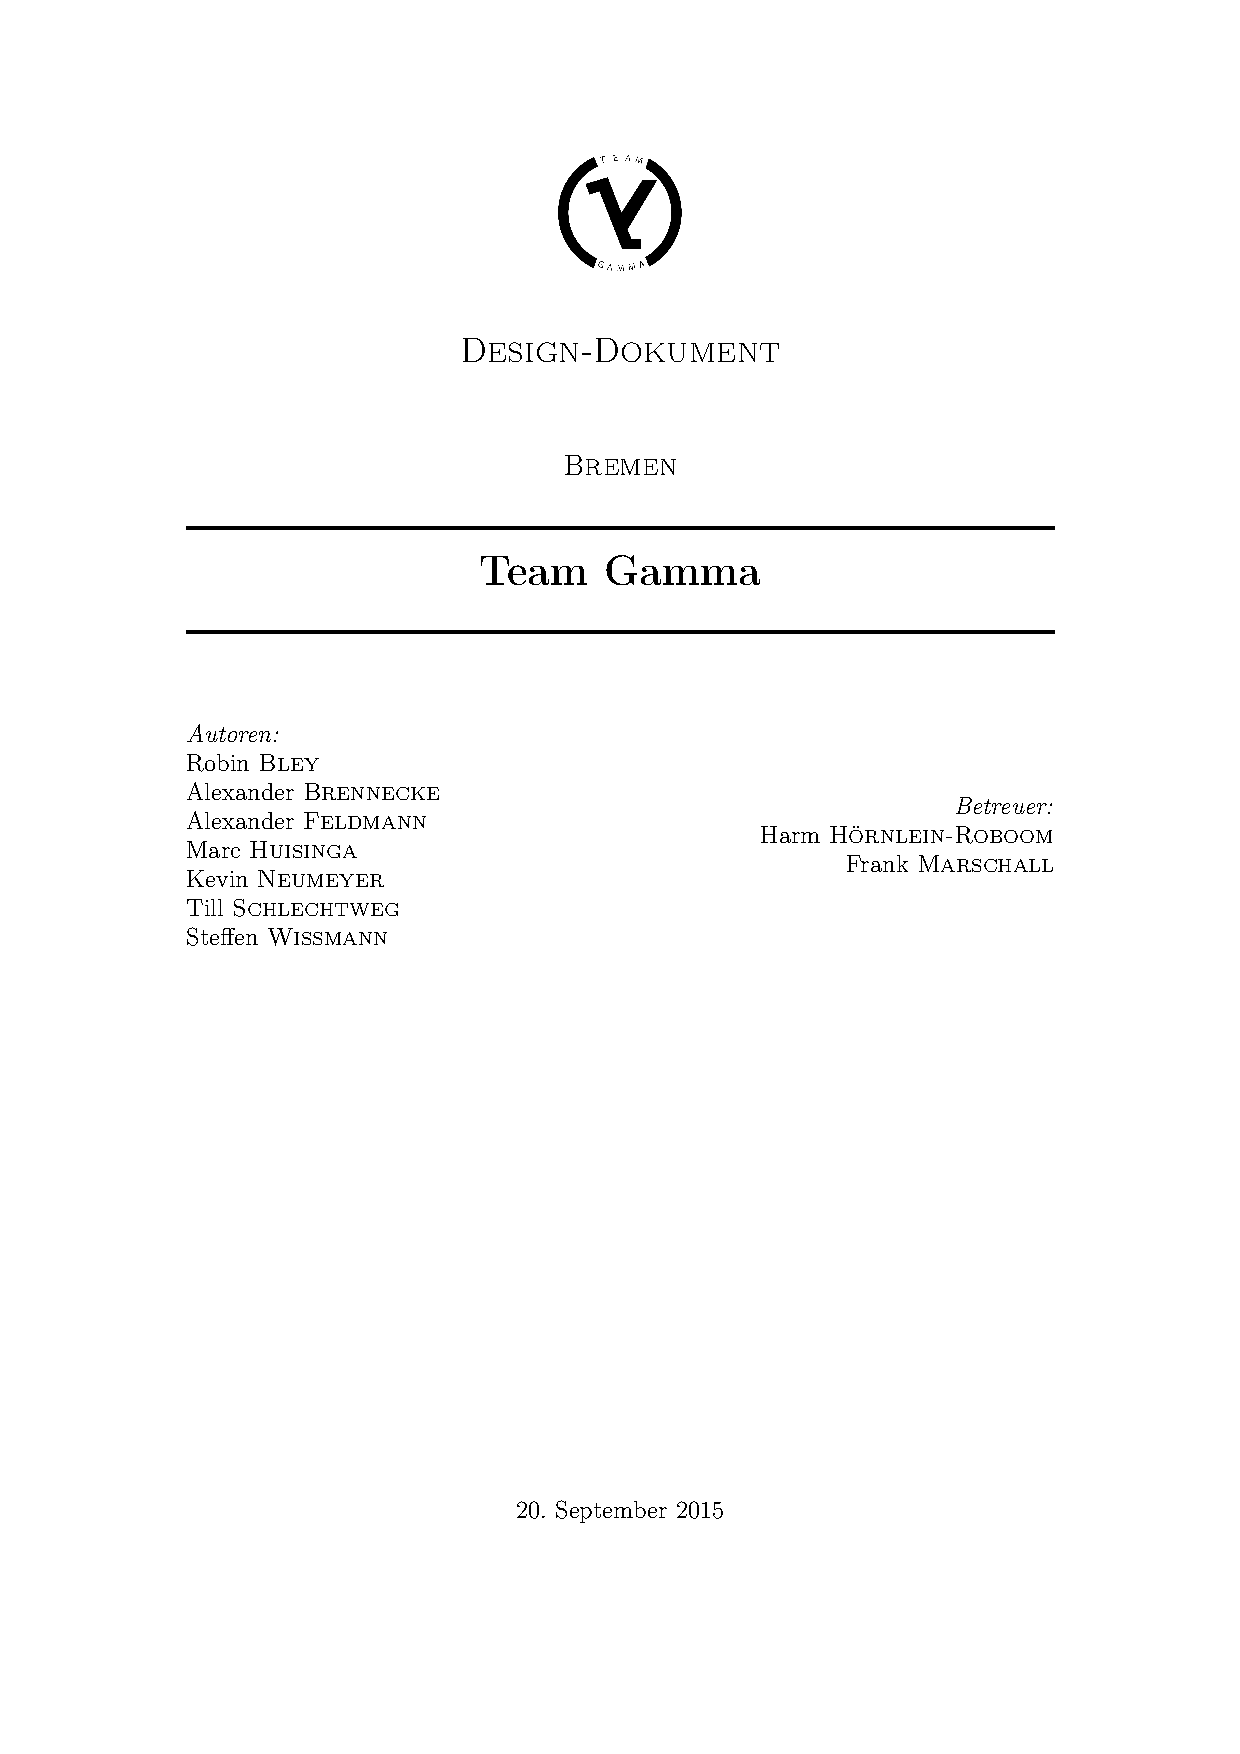
\includepdf [pages=-]{./4_Design_Document/design_document.pdf}

\end{document}